% Phase-space trajectory — pure TikZ (parametric).
\documentclass[border=4pt]{standalone}
\usepackage{tikz}
\usepackage{pgfplots}
\pgfplotsset{compat=1.18}

\definecolor{oiBlue}{HTML}{0072B2}
\definecolor{oiVerm}{HTML}{D55E00}
\definecolor{oiGreen}{HTML}{009E73}

\begin{document}
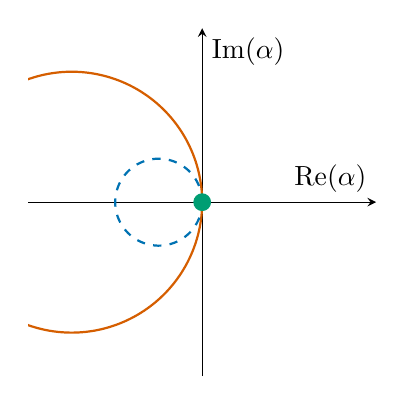
\begin{tikzpicture}
\begin{axis}[
    width=6cm, height=6cm,
    xlabel=$\mathrm{Re}(\alpha)$, ylabel=$\mathrm{Im}(\alpha)$,
    axis equal,
    axis lines=middle,
    xmin=-2, xmax=2, ymin=-2, ymax=2,
    xtick=\empty, ytick=\empty,
    font=\sffamily,
]
% Branch |r, down>: large loop
\addplot[oiVerm, thick, smooth, domain=0:360, samples=100]
  ({1.5*cos(x)-1.5}, {1.5*sin(x)});
% Branch |r, up>: stays at origin
\addplot[oiGreen, mark=*, only marks, mark size=3pt] coordinates {(0,0)};
% Branch |g, up>: small loop
\addplot[oiBlue, thick, smooth, dashed, domain=0:360, samples=100]
  ({0.5*cos(x)-0.5}, {0.5*sin(x)});
\end{axis}
\end{tikzpicture}
\end{document}
